\documentclass[oneside]{ntuthesis}

\usepackage{times}
\usepackage{verbatim}
\usepackage{color}
\usepackage{url}
\usepackage{graphicx}
\usepackage{array}
\usepackage{pdfpages} % include outside .pdf
\usepackage{wallpaper} % watermark


%%% Change chapter format + remove white strips %%%
\titleformat{\chapter}[hang]
{\normalfont\huge\bfseries}{\chaptertitlename~\thechapter}{20pt}{\Huge}
\titlespacing*{\chapter}{0pt}{50pt}{40pt}
\titlespacing*{name=\chapter,numberless}{0pt}{-30pt}{10pt}
%%%%%%%%%%%%%   END  %%%%%%%%%%%%


% Format the refs
\usepackage[sort,comma]{natbib}
\usepackage[hidelinks]{hyperref}

% For the tree
\usepackage{tikz}
\usepackage{tikz-qtree}

% For barchart
\usepackage{pgfplots}

% Using the tex-text mapping for ligatures etc.
\defaultfontfeatures{Mapping=tex-text}

% Set the default fonts
%\setmainfont{Times_New_Roman}
\setmainfont[Path = fonts/, BoldFont=TimesNewRomanBold.ttf, ItalicFont=TimesNewRomanItalic.ttf, BoldItalicFont=TimesNewRomanBoldItalic.ttf]{Times_New_Roman.ttf}
\usepackage{CJKutf8}
\setCJKmainfont[Path = fonts/, BoldFont=特粗楷體.TTC]{kaiu.ttf}


% Your information goes here
% author: Tz-Huan Huang [http://www.csie.ntu.edu.tw/~tzhuan]

% ----------------------------------------------------------------------------
% "THE CHOCOLATE-WARE LICENSE":
% Tz-Huan Huang wrote this file. As long as you retain this notice you
% can do whatever you want with this stuff. If we meet some day, and you think
% this stuff is worth it, you can buy me a chocolate in return Tz-Huan Huang
% ----------------------------------------------------------------------------

% Syntax: \var{English}{Chinese}
\university{National Taiwan University}{國立臺灣大學}
\college{College of Electrical Engineering and Computer Science}{電機資訊學院}
\institute{Graduate Institute of Communication Engineering}{電信工程學研究所}
\title{Road Extraction from Satellite Images Using Machine Learning Techniques}{Sujet en caraquetere}
\author{Alexandre Constantin}{康亞力}
\studentid{R06942123}
\advisor{Jian-Jiun Ding, Ph.D.}{丁建均\ 博士}
\defenseyear{2018}{107}
\defensemonth{July}{7}
\defenseday{31}


\begin{document}

% 臺大論文浮水印
% 臺大論文浮水印
\CenterWallPaper{0.174}{pdfs/watermark.pdf}
\setlength{\wpXoffset}{6.1725cm}
\setlength{\wpYoffset}{10.5225cm}


\hypersetup{pageanchor=false}

\frontmatter
\pagenumbering{gobble}
\makecover

\clearpages
\setcounter{page}{1}
\hypersetup{pageanchor=true}
\pagenumbering{roman}
\phantomsection

% generate certification
\makecertification
% or include scanned pdf
%\addcontentsline{toc}{chapter}{口試委員會審定書}
%
\includepdf[pages={1}]{pdfs/cert.pdf}

\begin{acknowledgementszh}
這是中文行距測試,應該看到一點五倍行距。這是中文行距測試,應該看到一點
五倍行距。這是中文行距測試,應該看到一點五倍行距。這是中文行距測試,應
該看到一點五倍行距。這是中文行距測試,應該看到一點五倍行距。這是中文行
距測試,應該看到一點五倍行距。這是中文行距測試,應該看到一點五倍行距。
這是中文行距測試,應該看到一點五倍行距。這是中文行距測試,應該看到一點
五倍行距。這是中文行距測試,應該看到一點五倍行距。這是中文行距測試,應
該看到一點五倍行距。這是中文行距測試,應該看到一點五倍行距。這是中文行
距測試,應該看到一點五倍行距。這是中文行距測試,應該看到一點五倍行距。

感謝\ldots
\end{acknowledgementszh}

\begin{acknowledgementsen}
%le temps passe vite, soudainement mes études à NTU terminent bientôt, je dois remercier premièrement mon tuteur professeur "DJJ", avec ses aides j'ai pu accompli cet article. Pendant ces deux ans de recherche, il m'a donné beaucoup de conseils sur la recherche, il m'a entraîné à partir de la base, pas à pas, les compétences face à la recherche, qui me permettent d'obtenir mon diplôme avec succès.

%d'ailleurs, je dois remercier aussi tout le monde de mon labo, merci mon ami blabla, et blabla, blabla, et blabla, blabla, et blabla, qui m'ont aidé avec leurs conseils et directions sur les cours et la recherche. Aussi mes collègues de master 2: blabla, et blabla, merci pour vos aides sur la vie quotidienne et vos accompagnements pendant ces deux ans de recherche. Merci pour les amis, blabla, et blabla, qui sont en master 1 d'avoir porter l'énergie dans le labo, j'espère que vous aurez un bon résultat sur la recherche.

%Et mes amis de lycée blabla, et blabla, merci d'avoir porté la bonheur pour moi quand j'étais déçu, je suis vraiment content de vous avoir en contact après avoit quitté le lycée..blablablabla

%et je dois remercier spécialement à ma famille, merci papa, maman, pour leur soutiens, et ma soeur qui vit aussi à taipei pour son accompagnement, j'espère que tu vas réussir ta vie, merci mon frère qui téléphone souvent pour me demander des nouvelles, qui m'a porté de la chaleur de la famille.

%d'ailleurs, merci xxx(je sais pas qui c'est, ça doit être les jurys)pour leur conseils, que j'ai pu améliorer cet article, merci à tout le monde, j'ai pas pu tout listé, mais je vous remercie avec tout mon coeur, grace à vous j'ai pu avancer et continuer dans ma direction de la vie.

%  (國立臺灣大學)    (電信工程學研究所)

Blabla bla texte sur plusieurs lignes. Blabla bla texte sur plusieurs lignes. Blabla bla texte sur plusieurs lignes. Blabla bla texte sur plusieurs lignes. Blabla bla texte sur plusieurs lignes. Blabla bla texte sur plusieurs lignes. Blabla bla texte sur plusieurs lignes.

\begin{flushright}
\\
June XX, 2018\\
National Taiwan University, MingDa Building, Room 531
\end{flushright}

\end{acknowledgementsen}

\begin{abstractzh}
這是中文行距測試,應該看到一點五倍行距。這是中文行距測試,應該看到一點
五倍行距。這是中文行距測試,應該看到一點五倍行距。這是中文行距測試,應
該看到一點五倍行距。這是中文行距測試,應該看到一點五倍行距。這是中文行
距測試,應該看到一點五倍行距。這是中文行距測試,應該看到一點五倍行距。
這是中文行距測試,應該看到一點五倍行距。這是中文行距測試,應該看到一點
五倍行距。這是中文行距測試,應該看到一點五倍行距。這是中文行距測試,應
該看到一點五倍行距。這是中文行距測試,應該看到一點五倍行距。這是中文行
距測試,應該看到一點五倍行距。這是中文行距測試,應該看到一點五倍行距。 \\

\noindent
關鍵字:台大、公館、羅斯福路、德田館
\end{abstractzh}

\begin{abstracten}
In computer vision, image classification always have an important place due to its widespread applications such as image compression, object tracking, image analysis and ground use evolution. In this particular area we will use classification to extract road networks from satellites images. It consists of giving a label to each pixel if it belongs or not to a road, the applications are very wide from Network mapping to monitor territories.

To extract the roads accurately we propose a machine learning based technique with additional classification algorithm as post-processing. Our procedure is described as follows: first the input image is cutted in small squares, it will fit better to a reduced neural network and will decrease computation time and provide more detailed information, we also increase the range of input data using color’s pre-processing algorithm. Then we exploit color channels and additional gradient channels to put inside the neural network that is trained to classify road and non-road pixels. Finally we verify with additional classification algorithm the detected roads and with post-processing complete the missing road parts to construct the final road map.

Simulations show that our proposed method detect most of the road pixels and outperforms state-of-the-art methods.\\

\noindent
\textbf{Index terms}: Satellite Images, Image classification, Computer Vision, Road Extraction, Machine Learning, Neural Network
\end{abstracten}


% Table of Content
\clearpages
\tableofcontents
% List of Figures
\clearpages
\listoffigures
% List of Tables
\clearpages
\listoftables

\mainmatter


%% CHANGE TOC FORMAT main chapters %%
\titlecontents{chapter}% <section-type>
  [0pt]% <left>
  {\bfseries}% <above-code>
  {\chaptername\ \thecontentslabel\quad}% <numbered-entry-format>
  {}% <numberless-entry-format>
  {\cftdotfill{\cftdotsep}\contentspage}% <filler-page-format>
%%%   End   %%%

% Your thesis goes here
\chapter{Introduction}
\label{c:intro}

The goal of this thesis is to detect roads and some other features. Automatic features extraction is still in research nowadays because of the complexity.
Road detection and feature detection are used in many fields for many applications such as:
\begin{itemize}
	\item{\textbf{Network mapping}: creating network database (road mapping, pipes analysis).}
	\item{\textbf{Ground analysis}: finding rural areas, forests: analysis of the ground occupation (ratios), inventory forests and see evolution. Agriculture with monitoring productions and geophysics with vaults analysis, ground deformation.}
	\item{\textbf{Defense}: monitoring territories, spying neighborhood or guidance systems (embedded data processing).}
	\item{\textbf{Risk prevention}: traffic monitoring, preventing risks and detect side-effects (after typhoon for example), sea surfaces monitoring or prediction of flooding.}
\end{itemize}

\section{Machine Learning and Road Extraction}

Road extraction is a comprehensively researched topic on data analysis, machine learning, and computer vision. There are over 20 million miles across the globe, and many of them have not yet been mapped. The general purpose of road extraction is to map areas of the world from aerial images to update maps more especially places with lower populatio and areas where there is frequent construction. With the aid of the data analysis tools in machine learning, computer can automatically recognize the scenario of the vision, the context of a conversation, or even aeras from images. Road extraction is an especially challenging problem because of the wide range of road colors and the similarity between roads area and other areas.

%%%% History part + references
% See thesis: start: Although face recognition is a lifelonf resaerch topic


\section{Motivation - Background}

\section{Contribution}

\section{Organization}

\textbf{CONSERV\'E POUR L'EXEMPLE}

Figure~\ref{i:cat}.
%i:cat
\begin{figure}[!htbp]
\centering
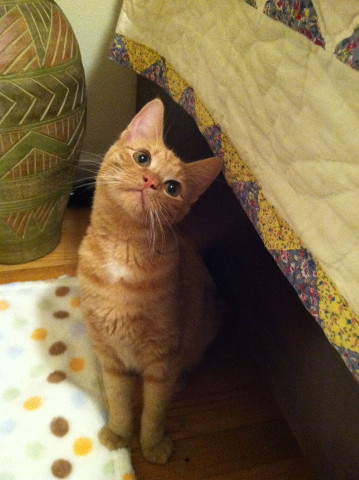
\includegraphics[width=0.58\textwidth]{images/cat}
\caption{A cat.}
\label{i:cat}
\end{figure}


As blabla pointed out, there were many videos~.%\citep{..}.


test \textbf{Test bold} et \textit{Test it} et \textbf{\textit{test BolDiT}}

\chapter{Related Work}
\label{c:related}

\section{First}
\label{s:related1}

This is English line spacing test. You should see double spacing text.
This is English line spacing test. You should see double spacing text.
This is English line spacing test. You should see double spacing text.
This is English line spacing test. You should see double spacing text.
This is English line spacing test. You should see double spacing text.
This is English line spacing test. You should see double spacing text.
This is English line spacing test. You should see double spacing text.
This is English line spacing test. You should see double spacing text.
This is English line spacing test. You should see double spacing text.
This is English line spacing test. You should see double spacing text.
This is English line spacing test. You should see double spacing text.
This is English line spacing test. You should see double spacing text.
This is English line spacing test. You should see double spacing text.
This is English line spacing test. You should see double spacing text.
This is English line spacing test. You should see double spacing text.
This is English line spacing test. You should see double spacing text.
This is English line spacing test. You should see double spacing text.
This is English line spacing test. You should see double spacing text.
This is English line spacing test. You should see double spacing text.
This is English line spacing test. You should see double spacing text.
This is English line spacing test. You should see double spacing text.
This is English line spacing test. You should see double spacing text.
This is English line spacing test. You should see double spacing text.
This is English line spacing test. You should see double spacing text.

\section{Second}

This is English line spacing test. You should see double spacing text.
This is English line spacing test. You should see double spacing text.
This is English line spacing test. You should see double spacing text.
This is English line spacing test. You should see double spacing text.
This is English line spacing test. You should see double spacing text.
This is English line spacing test. You should see double spacing text.
This is English line spacing test. You should see double spacing text.
This is English line spacing test. You should see double spacing text.
This is English line spacing test. You should see double spacing text.
This is English line spacing test. You should see double spacing text.
This is English line spacing test. You should see double spacing text.
This is English line spacing test. You should see double spacing text.
This is English line spacing test. You should see double spacing text.
This is English line spacing test. You should see double spacing text.
This is English line spacing test. You should see double spacing text.
As discussed in Section~\ref{s:related1} and Chapter~\ref{c:related}.

\chapter{Methods}
\label{c:method}

Our method is described in Algorithm~\ref{a:a1}.

\begin{algorithm}
    \caption{A Very Good Algorithm}
    \label{a:a1}
    \begin{algorithmic}[1]
        \Require  
            $I$: Something;
        \Ensure
            $O$: Something else;
        \State $S\gets$[]
        \Comment{Initialize $S$}
        \ForAll{Item $i$ {\bf in} $I$ }
            \State $S\gets$[]
            \Comment{Another comment}
        \EndFor
        \State \Return O
    \end{algorithmic}
\end{algorithm}

\chapter{Experiments}
\label{c:experiment}

There is a tree in Figure~\ref{i:tree}.
This is English line spacing test. You should see double spacing text.
This is English line spacing test. You should see double spacing text.
This is English line spacing test. You should see double spacing text.

%i:tree
\begin{figure}[!htbp]
\centering
\tikzset{every tree node/.style={align=center},
    level distance=40pt,
    sibling distance=6pt}
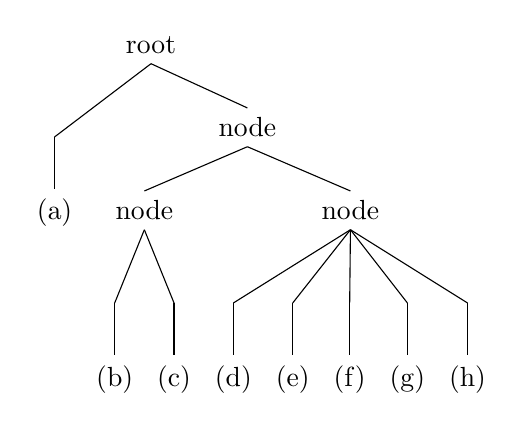
\begin{tikzpicture}
\Tree[.root
       [ (a) ]
       [.node
         [.node
           [ (b) ]
           [ (c) ]
         ]
         [.node
           [ (d) ]
           [ (e) ]
           [ (f) ]
           [ (g) ]
           [ (h) ]
         ]
       ]
     ]

\end{tikzpicture}

\caption{A tree. }
\label{i:tree}
\end{figure}


There is a barchart in Figure~\ref{i:barchart}.
This is English line spacing test. You should see double spacing text.
This is English line spacing test. You should see double spacing text.
This is English line spacing test. You should see double spacing text.

%i:barchart
\begin{figure}[!htbp]
    \centering
    \vspace{2em}
    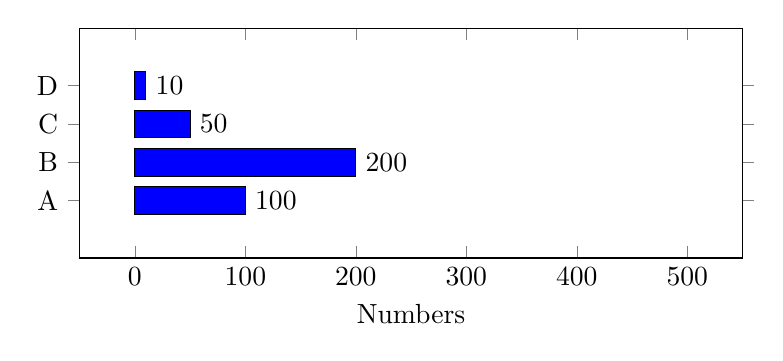
\begin{tikzpicture}
        \begin{axis}[
            enlarge y limits=0.5,
            enlarge x limits=0.1,
            height=4.5cm,
            width=10cm,
            symbolic y coords={A,B,C,D},
            xmin=0,
            xmax=500,
            xbar=1pt,
            xlabel=Numbers,
            nodes near coords={\pgfmathprintnumber[/pgf/number format/assume math mode]{\pgfplotspointmeta}},
            nodes near coords align={horizontal},
            every node near coord/.append style={
                anchor=west}
            ,
            xticklabel style={/pgf/number format/assume math mode},
            yticklabel style={/pgf/number format/assume math mode},
            ytick=data
          ]
            \addplot[xbar,fill=blue] coordinates {
            (100,A)
            (200,B)
            (50,C)
            (10,D)
            };
        \end{axis}
    \end{tikzpicture}
    \caption{A barchart.}
    \label{i:barchart}
\end{figure}


Our method outperforms state-of-art systems as shown in Table~\ref{t:results}.
This is English line spacing test. You should see double spacing text.
This is English line spacing test. You should see double spacing text.
This is English line spacing test. You should see double spacing text.

%t:results
\begin{table}[!htbp]
\centering
\begin{tabular}{|c|c|c|c|}
\hline

Method      &    Precision &     Recall &     F1-Score \\ \hline
their model &     3.40     &      3.40  &      3.40    \\ \hline
our model   &    99.99     &     99.99  &     99.99    \\ \hline


\end{tabular}
\caption{Final performance of our system. }
\label{t:results} 
\end{table}


\chapter{Conclusions}
\label{c:conclusion}


\clearpage
\appendix  % \@startappendix

%% CHANGE TOC FORMAT Appendix %%
\titlecontents{chapter}% <section-type>
  [0pt]% <left>
  {\bfseries}% <above-code>
  {\thecontentslabel\quad}% <numbered-entry-format>
  {}% <numberless-entry-format>
  {\cftdotfill{\cftdotsep}\contentspage}% <filler-page-format>
%%%   End   %%%


\chapter{Datasets}
\label{c:dataset}


\backmatter

%% CHANGE TOC FORMAT Bilbiography %%
\titlecontents{chapter}% <section-type>
  [0pt]% <left>
  {}% <above-code>
  {\chaptername\ \thecontentslabel\quad}% <numbered-entry-format>
  {}% <numberless-entry-format>
  {\cftdotfill{\cftdotsep}\contentspage}% <filler-page-format>
%%%   End   %%%

\clearpages
\phantomsection
\addcontentsline{toc}{chapter}{\bibname}
\bibliographystyle{apa}

% Your bibliography goes here
\bibliography{thesis}

\end{document}
